\documentclass[paper=a4, fontsize=11pt]{scrartcl} % A4 paper and 11pt font size
\usepackage{./../usfassignment}
\settitle{Assignment 6}
\setauthor{Wanzhang Sheng}
\setcourse{CS675: Automata Theory}

\begin{document}

\maketitle % Print the title

% -----------------------------------------------------------------------------
% PROBLEM 1
% -----------------------------------------------------------------------------
\section{}

\begin{fancyquotes}
  For each language $L$, if:
  \begin{itemize}
  \item $L$ is regular, give a regular expression and a finite
    automaton (either deterministic or non-deterministic) for $L$
  \item $L$ is context-free (but not regular), prove that $L$ is not
    regular using the pumping lemma, and give a Context-Free Grammar
    for $L$ and give a push-down automata for $L$
  \item $L$ is not context-free, prove that $L$ is not Context-Free
    using the context-free pumping lemma (and possibly closure
    properties).
  \end{itemize}
\end{fancyquotes}

\begin{enumerate}
\item
  \begin{fancyquotes}
    $\{a^{2n} : n>0\}$
  \end{fancyquotes}


  $L$ is regular as $(aa)^*aa$.

  \begin{figure*}[hp]
    \centering
    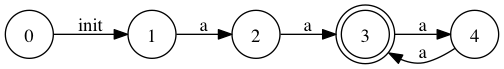
\includegraphics[width=0.6\textwidth]{6-1.gv.png}
    \caption{$\{a^{2n} : n>0\}$}
  \end{figure*}

\item
  \begin{fancyquotes}
    $\{a^{2^n} : n>0\}$
  \end{fancyquotes}


  $L$ is not context-free.

  Assume $L$ is context-free.

  Let $n = 2^m, m>0$ be the constant of the Context-Free pumping
  lemma.

  Given $w = a^{n}$, we can break $w = uvxyz$,
  which $0<|vy|=k<n$. Then $|uxz| = n-k$, and $uv^{i}xy^{i}z =
  a^{n+(i-1)k}$.

  Then let $i=2$, so that $w=a^{2^{m}+k}$.
  Since $k<n=2^{m}$, then $2^{m}+k<2\times 2^{m}=2^{m+1}$.
  Which $a^{2^{m+1}}$ is the shortest one longer than $a^{2^m}$.
  So $w = a^{2^{m}+k}\not\in L$.

  So $L$ is not context-free.

\item
  \begin{fancyquotes}
    $\{a^{n}b^{m} : m\leq n\leq 2m \}$
  \end{fancyquotes}

  Assume $L$ is regular.

  Let $n$ be the constant of the pumping lemma.

  Given string $w = a^{n}b^{n}$, we can break into $xyz$, which
  $|xy|<n, |y|>0$. So $y$ must be all $0$'s, let $y = a^{j}$.

  Consider when $i=0$. $w_2 = xy^{0}z = a^{n-j}b^{n}\not\in L$.

  So $L$ is not regular.

  Context-Free Grammer:

  \[
  S \rightarrow aSb | aaSb | \epsilon
  \]

  PDA:
  \begin{figure}[hp]
    \centering
    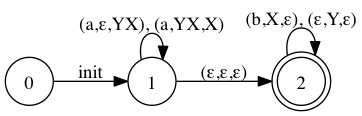
\includegraphics[scale=0.7]{6-1.gv.2.png}
    \caption{$\{a^{n}b^{m} : m\leq n\leq 2m \}$}
  \end{figure}

\end{enumerate}

\pagebreak

\end{document}
%%% Local Variables:
%%% mode: latex
%%% TeX-master: t
%%% End:
